% ------------------------------------------------------------------------------
% TYPO3 CMS 6.2 LTS - What's New - Chapter "Backend Changes" (Italian Version)
%
% @author Roberto Torresani <roberto.torresani@typo3.org>
% @license	Creative Commons BY-NC-SA 3.0
% @link		http://typo3.org/download/release-notes/whats-new/
% @language	Italian
% ------------------------------------------------------------------------------
% Chapter: Backend Changes
% ------------------------------------------------------------------------------

\section{Cambiamenti nel backend}
\begin{frame}[fragile]
	\frametitle{Cambiamenti nel backend}

	\begin{center}\huge{Capitolo 3:}\end{center}
	\begin{center}\huge{\color{typo3darkgrey}\textbf{Cambiamenti nel backend}}\end{center}

\end{frame}

% ------------------------------------------------------------------------------
% Autofocus
% ------------------------------------------------------------------------------
% http://forge.typo3.org/issues/49228

\begin{frame}[fragile]
	\frametitle{Cambiamenti nel backend}
	\framesubtitle{Backend Login}

 	\begin{itemize}
		\item Autofocus sul campo username nel form di login al backend\newline
			(attributo HTML5: \texttt{autofocus="autofocus"})
	\end{itemize}

	\begin{figure}
		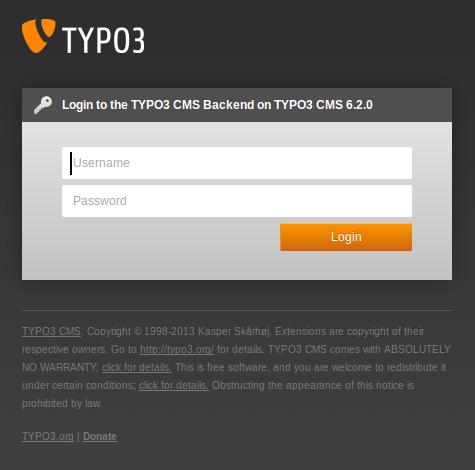
\includegraphics[width=0.4\linewidth]{Images/BackendChanges/BackendLogin.png}
	\end{figure}

\end{frame}

% ------------------------------------------------------------------------------
% Visual Appearance
% ------------------------------------------------------------------------------
% http://forge.typo3.org/issues/48376

\begin{frame}[fragile]
	\frametitle{Cambiamenti nel backend}
	\framesubtitle{Aspetto grafico}

	\begin{columns}[T]

		\begin{column}{.5\textwidth}
			\begin{itemize}
				\item Migliorata l'usabilità rivedendo gli spazi
				\item Aumentati gli spazi tra i moduli (colonna elenco di sinistra)
				\item E' basato su una griglia a 12px, che è stata raddoppiata
			\end{itemize}

			\advance\leftskip+3.0cm

			\smaller
				Sinistra: TYPO3 4.5\newline
				Destra: TYPO3 6.2
			\normalsize
		\end{column}

		\begin{column}{.5\textwidth}
			\begin{figure}\vspace*{-0.4cm}
				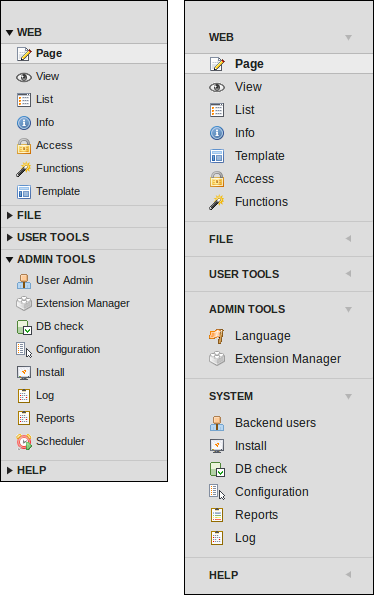
\includegraphics[width=0.6\linewidth]{Images/BackendChanges/VisualAppearance.png}
			\end{figure}
		\end{column}

	\end{columns}

\end{frame}

% ------------------------------------------------------------------------------
% Visual Appearance
% ------------------------------------------------------------------------------

\begin{frame}[fragile]
	\frametitle{Cambiamenti nel backend}
	\framesubtitle{Aspetto grafico}

	\begin{columns}[T]

		\begin{column}{.6\textwidth}

			\begin{itemize}
				\item Ristrutturati i moduli nella colonna di sinistra
				\item Il modulo "STRUMENTI DI AMMINISTRAZIONE" è stato diviso in due parti:

					\begin{itemize}
						\item \textbf{STRUMENTI DI AMMINISTRAZIONE} ("Linguaggio" e "Gestione estensioni")
						\item \textbf{SISTEMA} (strumenti di basso livello, che non mostrano le tre colonne della pagina)
					\end{itemize}

				\item Il modulo "TypoScript Help" è stato rimosso (obsoleto)

			\end{itemize}

		\end{column}

		\begin{column}{.4\textwidth}
			\begin{figure}\vspace*{-0.4cm}
				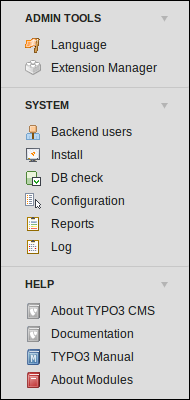
\includegraphics[width=0.35\linewidth]{Images/BackendChanges/AdminTools.png}
			\end{figure}
		\end{column}

	\end{columns}

\end{frame}

% ------------------------------------------------------------------------------
% Visual Appearance
% ------------------------------------------------------------------------------
% http://forge.typo3.org/issues/36017

\begin{frame}[fragile]
	\frametitle{Cambiamenti nel backend}
	\framesubtitle{Aspetto grafico}

	\begin{itemize}
		\item Il titolo \texttt{<h1>} nell'area principale utilizza il font "Share"
	\end{itemize}

	\begin{figure}
		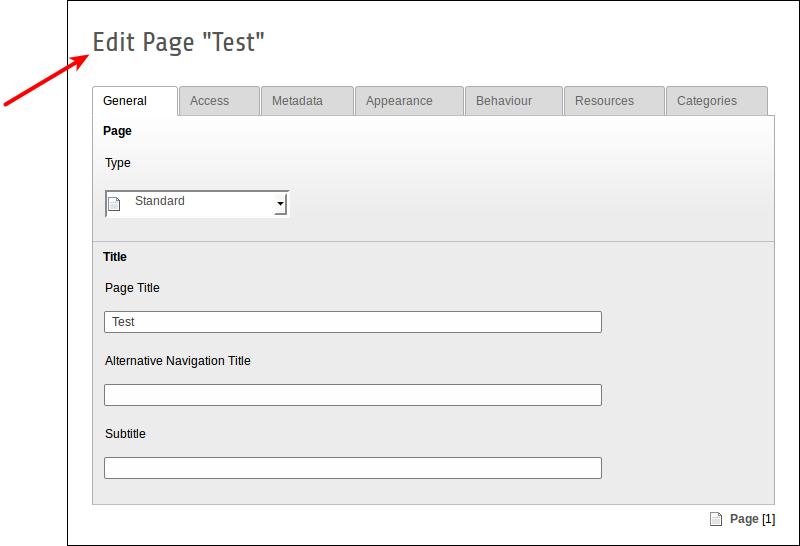
\includegraphics[width=0.6\linewidth]{Images/BackendChanges/ConsistantFont.png}
	\end{figure}

\end{frame}

% ------------------------------------------------------------------------------
% Visual Appearance
% ------------------------------------------------------------------------------
% http://forge.typo3.org/issues/41631

\begin{frame}[fragile]
	\frametitle{Cambiamenti nel backend}
	\framesubtitle{Aspetto grafico}

	\begin{itemize}
		\item Il modulo "Reports" ha una nuova icona
	\end{itemize}

	\begin{figure}
		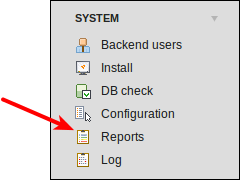
\includegraphics[width=0.35\linewidth]{Images/BackendChanges/ModuleReportsIcon.png}
	\end{figure}

\end{frame}

% ------------------------------------------------------------------------------
% Drag&Drop File Upload in Filelist (FAL)
% ------------------------------------------------------------------------------
% http://forge.typo3.org/issues/47005

\begin{frame}[fragile]
	\frametitle{Cambiamenti nel backend}
	\framesubtitle{Caricamento file con Drag\&Drop (1)}

	\begin{itemize}
		\item La funzionalità Drag\&Drop dell'HTML5 per il caricamento di file è stata implementata nella lista file

	\end{itemize}

	\begin{figure}
		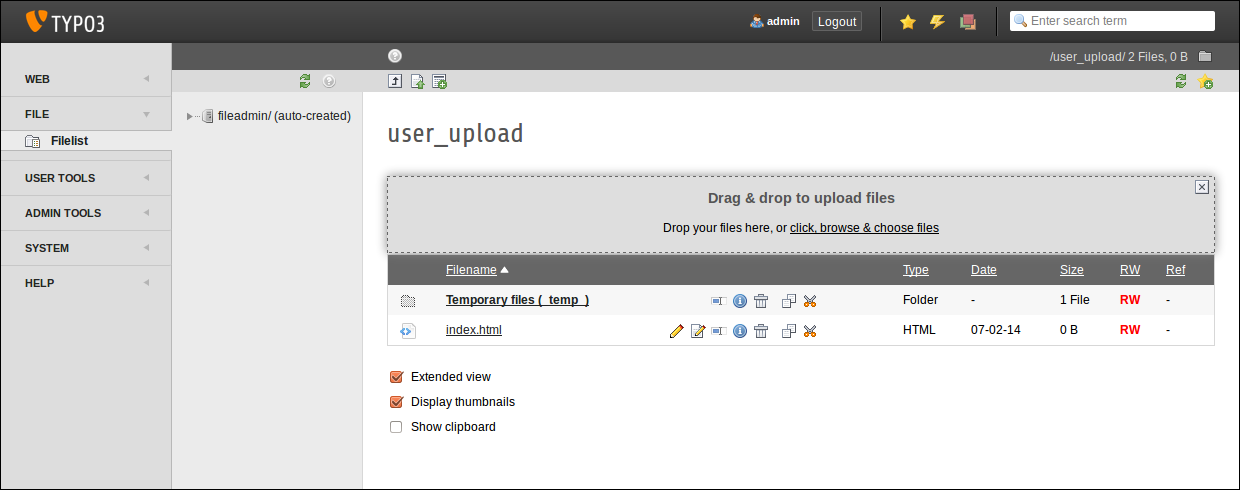
\includegraphics[width=0.95\linewidth]{Images/BackendChanges/DragDropFileUpload.png}
	\end{figure}

\end{frame}

% ------------------------------------------------------------------------------
% Drag&Drop File Upload Via Content Elements
% (slide added in March 2014)
% ------------------------------------------------------------------------------

\begin{frame}[fragile]
	\frametitle{Cambiamenti nel backend}
	\framesubtitle{Caricamento file con Drag\&Drop (2)}

	\begin{itemize}
		\item ...possibile anche con l'elemento di contenuto (bottone: "Scegli \& carica file")

	\end{itemize}

	\begin{figure}
		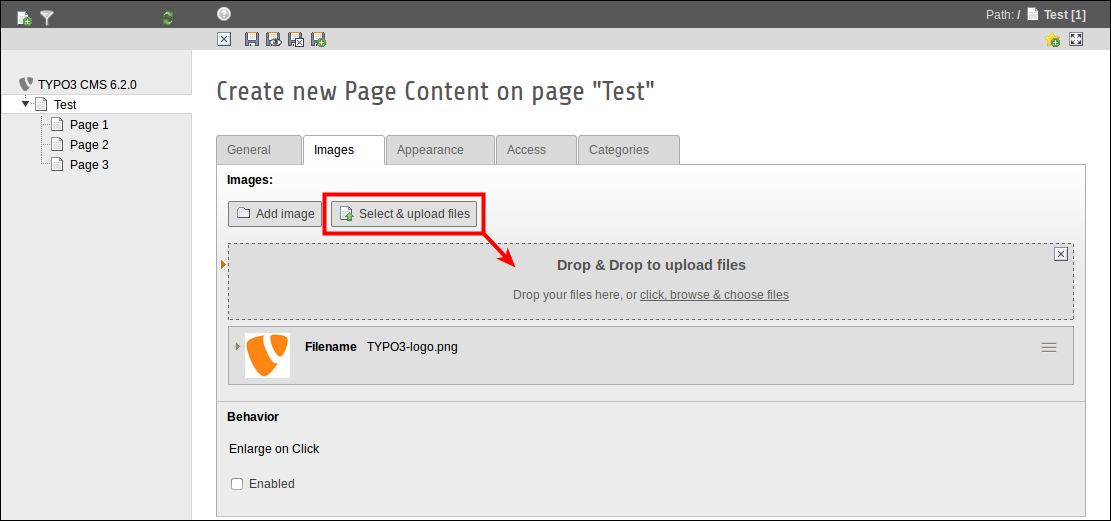
\includegraphics[width=0.95\linewidth]{Images/BackendChanges/SelectAndUploadFiles.png}
	\end{figure}

\end{frame}

% ------------------------------------------------------------------------------
% Backend Users
% ------------------------------------------------------------------------------
% http://forge.typo3.org/issues/43053

\begin{frame}[fragile]
	\frametitle{Cambiamenti nel backend}
	\framesubtitle{Usabilità: Lista utenti di Backend}

	\begin{itemize}
		\item Username e nome reale sono mostrati (prima colonna nella lista)
		\item Clicca sul link del (user)name per editare il record
		\item Aggiunto il bottone Cancella alla lista

	\end{itemize}

	\begin{figure}
		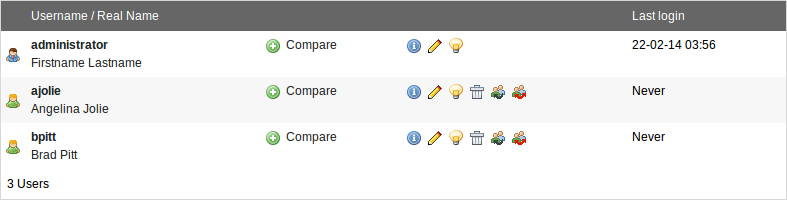
\includegraphics[width=0.95\linewidth]{Images/BackendChanges/BackendUserList.png}
	\end{figure}

\end{frame}

% ------------------------------------------------------------------------------
% Live Search
% ------------------------------------------------------------------------------
% http://forge.typo3.org/issues/35358

\begin{frame}[fragile]
	\frametitle{Cambiamenti nel backend}
	\framesubtitle{Ricerca in linea}

	\begin{itemize}
		\item Il tooltip mostra l'UID e il PID nei risultati della ricerca
		\item Quando, dopo una ricerca, si chiude il modulo per la ricerca, è mostrata la lista ad elenco della pagina (non una pagina vuota)
	\end{itemize}

	\begin{figure}
		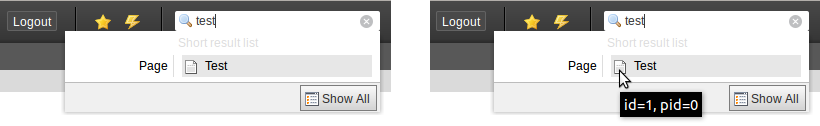
\includegraphics[width=0.8\linewidth]{Images/BackendChanges/LiveSearchTooltip.png}
	\end{figure}

\end{frame}

% ------------------------------------------------------------------------------
% Live Search
% ------------------------------------------------------------------------------

\begin{frame}[fragile]
	\frametitle{Cambiamenti nel backend}
	\framesubtitle{Ricerca in linea}

	\begin{itemize}
		\item In TYPO3 < 6.2, per le pagine, solo i campi del database \texttt{title} e \texttt{uid} sono utilizzati per la ricerca
		\item In TYPO3 >= 6.2, il campo \texttt{alias} può essere aggiunto alla ricerca\newline
			(richiede UserTSconfig: \texttt{options.pageTree.searchInAlias = 1})
	\end{itemize}

	\begin{figure}
		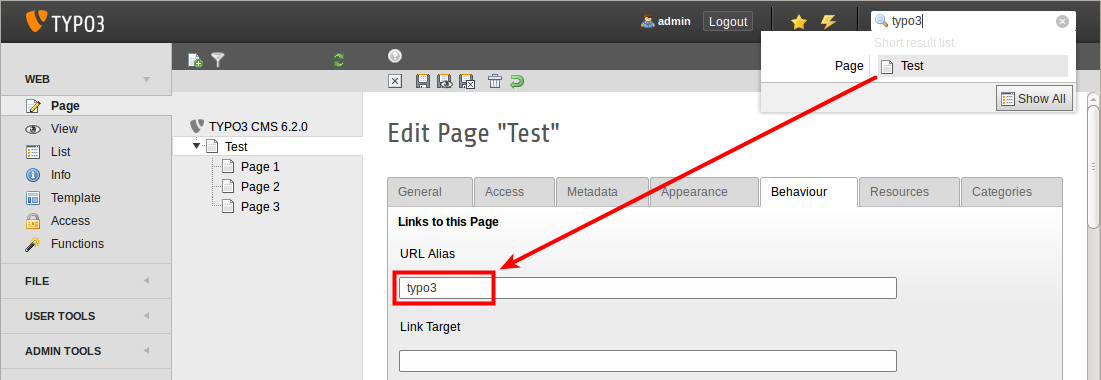
\includegraphics[width=0.95\linewidth]{Images/BackendChanges/LiveSearchInAlias.png}
	\end{figure}

\end{frame}

% ------------------------------------------------------------------------------
% File Abstraction Layer
% ------------------------------------------------------------------------------

\begin{frame}[fragile]
	\frametitle{Cambiamenti nel backend}
	\framesubtitle{File Abstraction Layer}

	\begin{itemize}
		\item Il titolo e il nome del file sono mostrati nell'intestazione dell'elemento FAL
	\end{itemize}

	\begin{figure}
		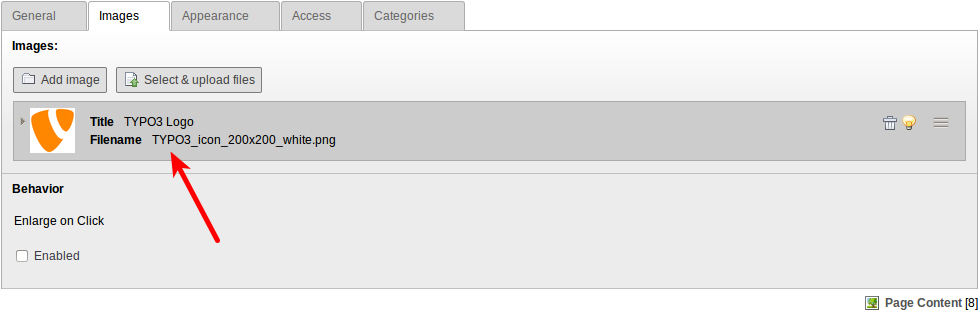
\includegraphics[width=0.95\linewidth]{Images/BackendChanges/FalTitleAndFilename.png}
	\end{figure}

\end{frame}

% ------------------------------------------------------------------------------
% File Abstraction Layer
% ------------------------------------------------------------------------------

\begin{frame}[fragile]
	\frametitle{Cambiamenti nel backend}
	\framesubtitle{File Abstraction Layer (EXT:filemetadata)}

	\begin{itemize}
		\item L'estensione di sistema "filemetadata" aggiunge dei tab per gestire i metadata
			\small(l'estensione è presente ma non caricata di default)\normalsize
	\end{itemize}

	\begin{figure}
		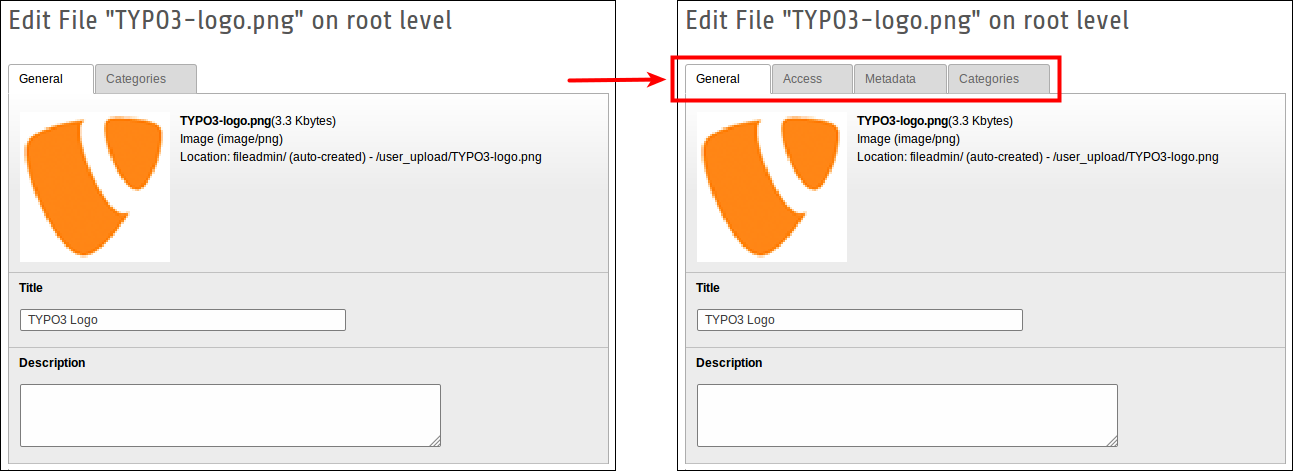
\includegraphics[width=0.95\linewidth]{Images/BackendChanges/FileMetaDataTabs.png}
	\end{figure}

\end{frame}

% ------------------------------------------------------------------------------
% File Abstraction Layer
% ------------------------------------------------------------------------------

\begin{frame}[fragile]
	\frametitle{Cambiamenti nel backend}
	\framesubtitle{File Abstraction Layer (EXT:filemetadata)}

	\begin{figure}
		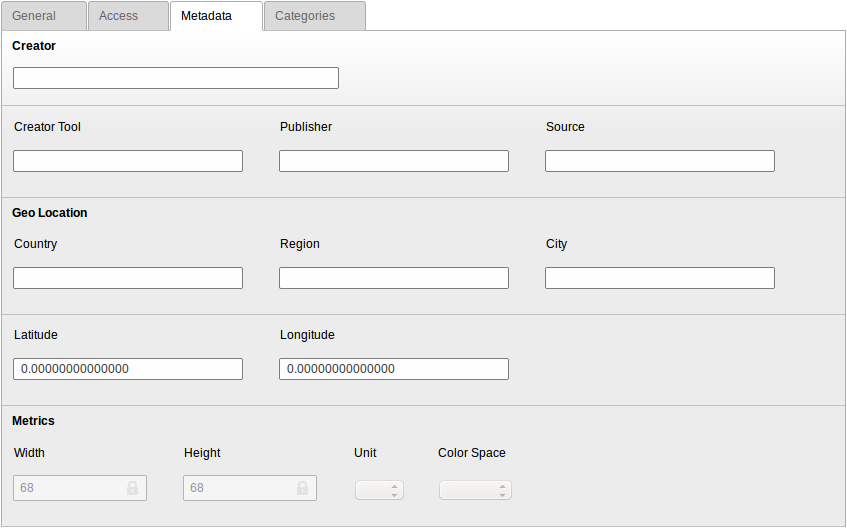
\includegraphics[width=0.8\linewidth]{Images/BackendChanges/FileMetaData.png}
	\end{figure}

\end{frame}

% ------------------------------------------------------------------------------
% File Abstraction Layer
% ------------------------------------------------------------------------------

\begin{frame}[fragile]
	\frametitle{Cambiamenti nel backend}
	\framesubtitle{File Abstraction Layer}

	\begin{itemize}
		\item Ora è possibile tradurre i metadata del FAL nei linguaggi usati nel frontend
	\end{itemize}

	\begin{figure}
		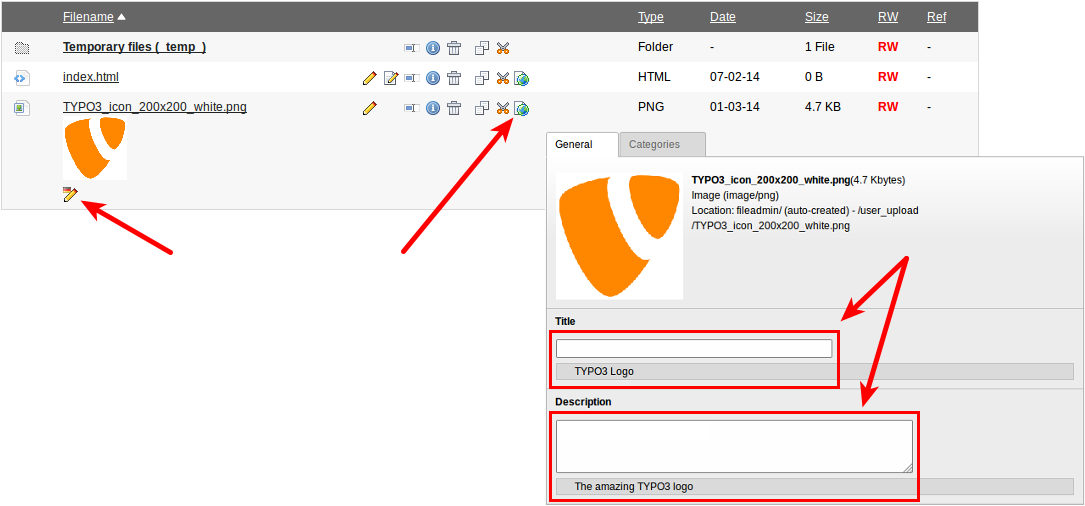
\includegraphics[width=0.95\linewidth]{Images/BackendChanges/FalTranslateMetaData.png}
	\end{figure}

\end{frame}

% ------------------------------------------------------------------------------
% Module: Documentation
% ------------------------------------------------------------------------------

\begin{frame}[fragile]
	\frametitle{Cambiamenti nel backend}
	\framesubtitle{Modulo: Documentazione}

	\begin{columns}[T]

		\begin{column}{.5\textwidth}
			\begin{itemize}
				\item Il modulo "Documentazione" permette agli utenti di scaricare e visualizzare i manuali
				\item La nuova installazione di TYPO3 carica questo modulo di default
				\item "Scarica documentazione" permette di scaricare i manuali (vedi foto)
				\item Usa l'Extension Manager per caricare il modulo "documentazione" in un aggiornamento di TYPO3
			\end{itemize}
		\end{column}

		\begin{column}{.5\textwidth}
			\begin{figure}\vspace*{-0.4cm}
				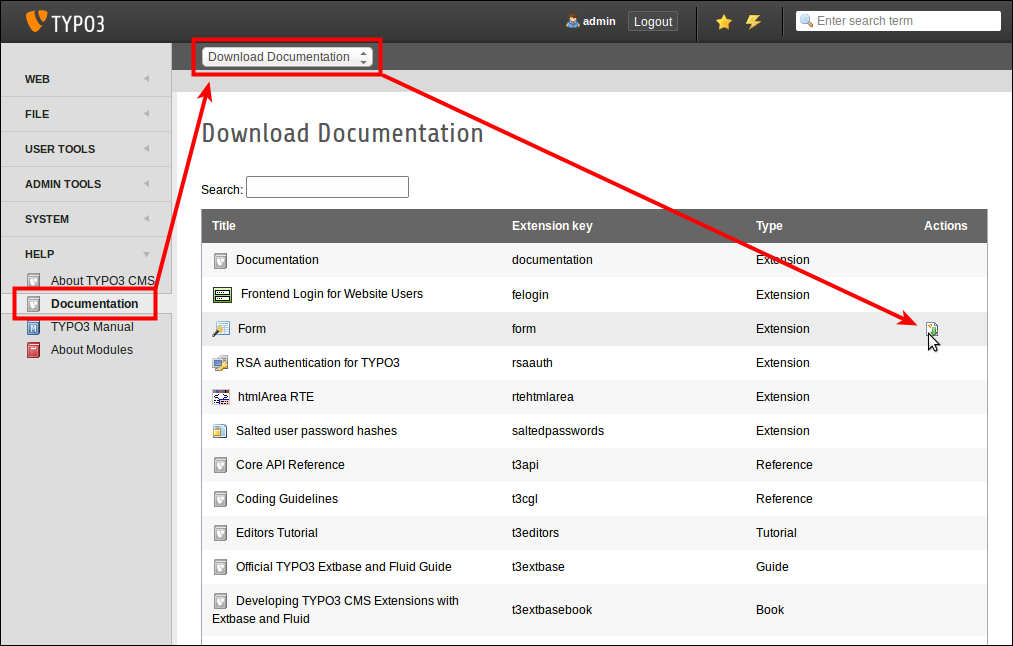
\includegraphics[width=1\linewidth]{Images/BackendChanges/DownloadDocumentation.png}
			\end{figure}
		\end{column}

	\end{columns}

\end{frame}

% ------------------------------------------------------------------------------
% Module: Documentation
% ------------------------------------------------------------------------------

\begin{frame}[fragile]
	\frametitle{Cambiamenti nel backend}
	\framesubtitle{Modulo: Documentazione}

	\begin{itemize}
		\item La funzione "Mostra documentazione" visualizza i manuali scaricati
	\end{itemize}

	\begin{figure}
		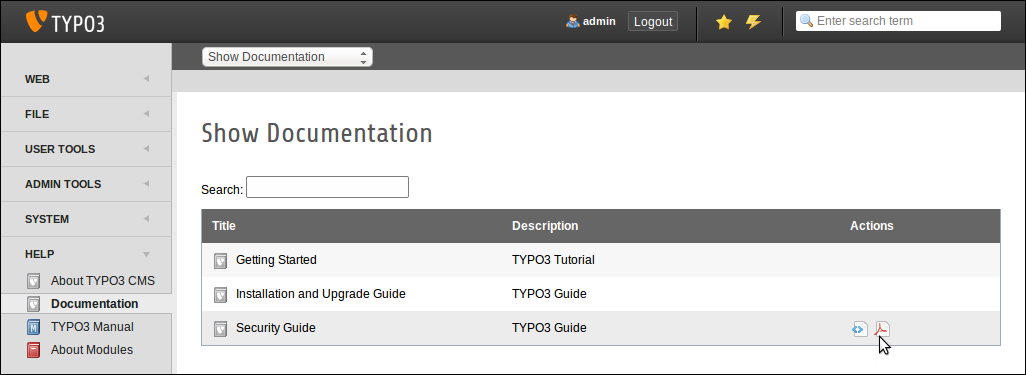
\includegraphics[width=0.95\linewidth]{Images/BackendChanges/ShowDocumentation.png}
	\end{figure}

\end{frame}

% ------------------------------------------------------------------------------
% Removed: TypoScript Help
% ------------------------------------------------------------------------------
% http://forge.typo3.org/issues/47931

\begin{frame}[fragile]
	\frametitle{Cambiamenti nel backend}
	\framesubtitle{Rimosso: TypoScript Help}

 	\begin{itemize}
		\item EXT:tsconfig\_help ("TSconfig Quick Reference") è stato rimosso\newline
			\small(informazioni non aggiornate dalla versione TYPO3 CMS 4.1)
	\end{itemize}

	\begin{figure}
		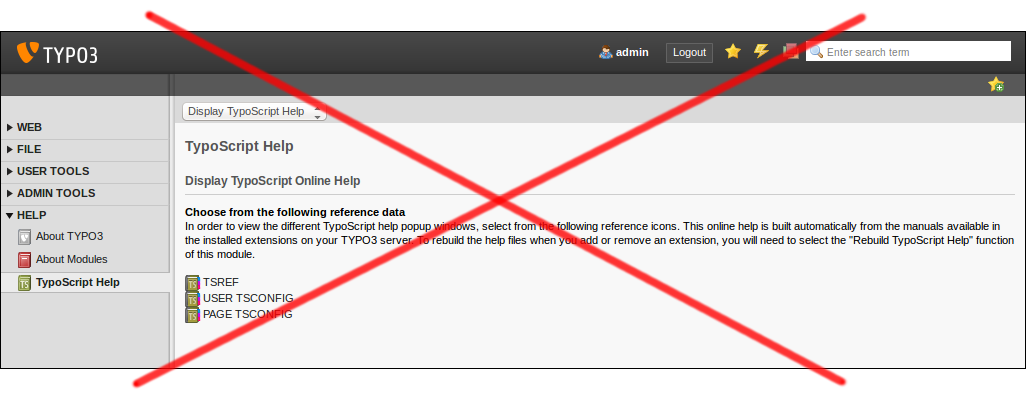
\includegraphics[width=0.95\linewidth]{Images/BackendChanges/TypoScriptHelpRemovedCrossed.png}
	\end{figure}

\end{frame}


% ------------------------------------------------------------------------------
% Scheduler
% ------------------------------------------------------------------------------

\begin{frame}[fragile]
	\frametitle{Cambiamenti nel backend}
	\framesubtitle{Scheduler}

	\begin{itemize}
		\item Possibilità di cancellare un task dello scheduler nella visualizzazione di dettaglio
			\small(in TYPO3 < 6.2, la funziona cancella era disponibile solo nella vista ad elenco)\normalsize
	\end{itemize}

	\begin{figure}
		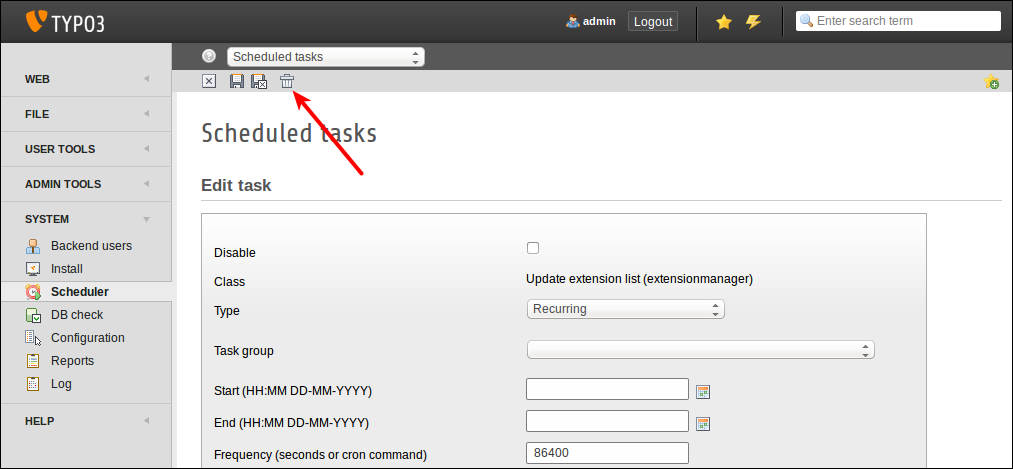
\includegraphics[width=0.95\linewidth]{Images/BackendChanges/DeleteSchedulerTaskInEditView.png}
	\end{figure}

\end{frame}

% ------------------------------------------------------------------------------
% Scheduler
% ------------------------------------------------------------------------------

\begin{frame}[fragile]
	\frametitle{Cambiamenti nel backend}
	\framesubtitle{Scheduler}

	\begin{itemize}
		\item Può essere inserita una descrizione nei task dello scheduler e sono visualizzate come sottotitoli nell'elenco, o come tooltip (vedi prossima slide)
	\end{itemize}

	\begin{figure}
		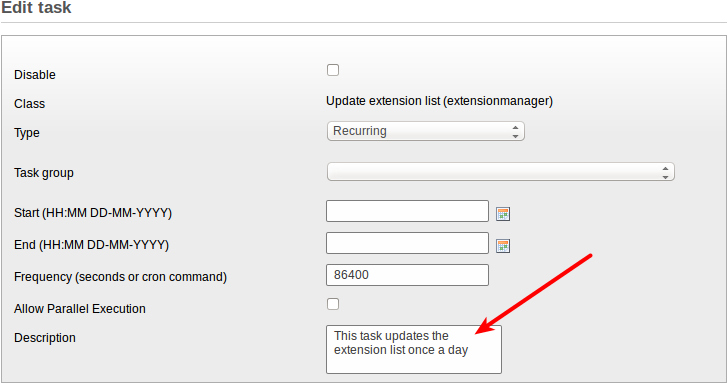
\includegraphics[width=0.7\linewidth]{Images/BackendChanges/SchedulerTaskDescription.png}
	\end{figure}

\end{frame}

% ------------------------------------------------------------------------------
% Scheduler
% ------------------------------------------------------------------------------

\begin{frame}[fragile]
	\frametitle{Cambiamenti nel backend}
	\framesubtitle{Scheduler}

	\begin{itemize}
		\item Descrizione del task come sottotitolo\newline
			\small(questa funziona va attivata nella configurazione dell'estensione)\normalsize
	\end{itemize}

	\begin{figure}
		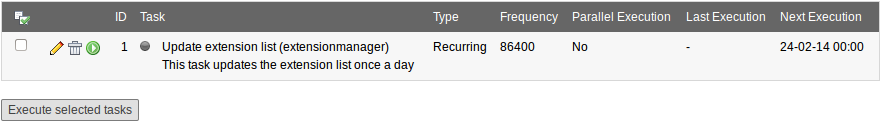
\includegraphics[width=0.95\linewidth]{Images/BackendChanges/SchedulerTaskDescriptionAsSubheader.png}
	\end{figure}

	\begin{itemize}
		\item Descrizione del task come tooltip ("hover")
	\end{itemize}

	\begin{figure}
		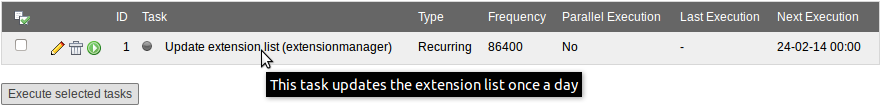
\includegraphics[width=0.95\linewidth]{Images/BackendChanges/SchedulerTaskDescriptionAsTooltip.png}
	\end{figure}

\end{frame}

% ------------------------------------------------------------------------------
% Scheduler
% ------------------------------------------------------------------------------

\begin{frame}[fragile]
	\frametitle{Cambiamenti nel backend}
	\framesubtitle{Scheduler}

        \begin{itemize}
                \item E' possibile raggruppare i task dello scheduler
                \item Aggiungi "scheduler task group" record alla pagina root (UID: 0)\newline
                        e seleziona gruppo nel task
        \end{itemize}


	\begin{figure}
		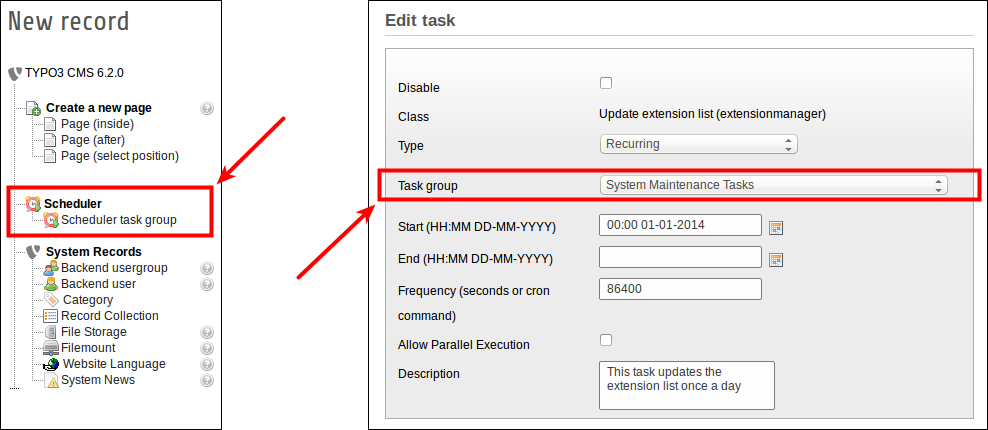
\includegraphics[width=0.95\linewidth]{Images/BackendChanges/SchedulerTaskGroup.png}
	\end{figure}

\end{frame}

% ------------------------------------------------------------------------------
% System Extension: Form
% ------------------------------------------------------------------------------
% http://forge.typo3.org/issues/38094

\begin{frame}[fragile]
	\frametitle{Cambiamenti nel backend}
	\framesubtitle{System Extension: Form}

	\begin{columns}[T]

		\begin{column}{.5\textwidth}
			\begin{itemize}
				\item Nuovo post-processor per il cObject FORM: \textbf{redirect}\newline
					(redirect dopo l'invio del form)
				\item Il valore è passato da \texttt{typolink} (funzione TypoScript),\newline
					il che significa che il valore può essere un ID di pagina o un URL
			\end{itemize}
		\end{column}

		\begin{column}{.5\textwidth}
			\begin{figure}\vspace*{-0.4cm}
				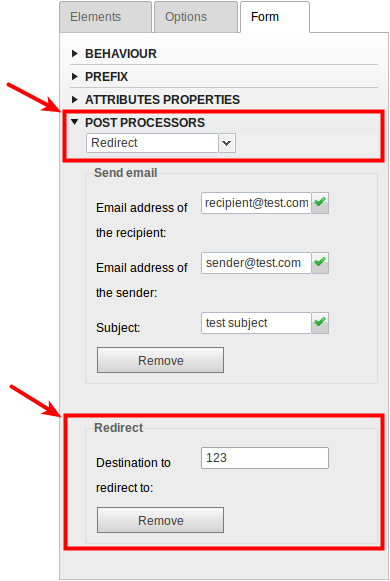
\includegraphics[width=0.65\linewidth]{Images/BackendChanges/FormRedirectPostProcessor.png}
			\end{figure}
		\end{column}

	\end{columns}

\end{frame}

% ------------------------------------------------------------------------------
% Module: List
% ------------------------------------------------------------------------------
% http://forge.typo3.org/issues/49810

\begin{frame}[fragile]
	\frametitle{Cambiamenti nel backend}
	\framesubtitle{List Module}

	\begin{itemize}
		\item Aggiunte le colonne "UID" e "PID" nella vista a lista per i non amministratori
	\end{itemize}

	\begin{figure}
		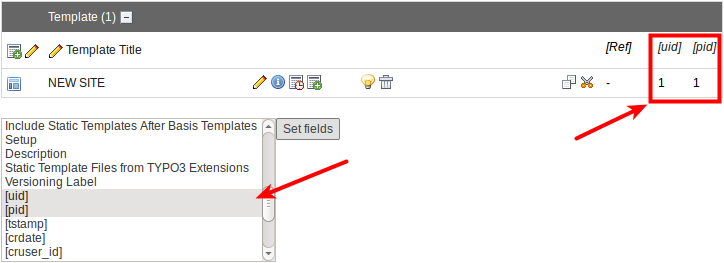
\includegraphics[width=0.95\linewidth]{Images/BackendChanges/AdditionalColumnsInListModule.png}
	\end{figure}

\end{frame}

% ------------------------------------------------------------------------------
% File Abstraction Layer
% ------------------------------------------------------------------------------
% http://forge.typo3.org/issues/50827
% http://forge.typo3.org/issues/51097

\begin{frame}[fragile]
	\frametitle{Cambiamenti nel backend}
	\framesubtitle{File Abstraction Layer}

	\begin{itemize}
		\item Se l'indexer trova un file mancante, un messaggio è visualizzato e un flag nel record del database è impostato
		\item Il modulo "Reports" segnala questa situazione
		\item Quando il file è nuovamente presente, il messaggio e il flag sono azzerati
	\end{itemize}

	\begin{columns}[T]

		\begin{column}{.5\textwidth}
			\begin{figure}
				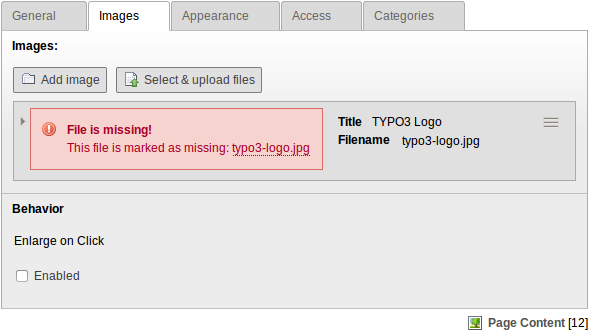
\includegraphics[width=0.95\linewidth]{Images/BackendChanges/FalMissingFileContentElement.png}
			\end{figure}
		\end{column}

		\begin{column}{.5\textwidth}
			\begin{figure}
				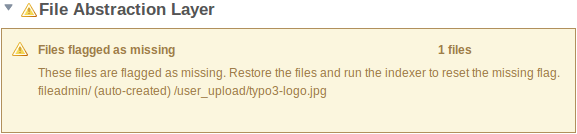
\includegraphics[width=0.95\linewidth]{Images/BackendChanges/FalMissingFileReportsModule.png}
			\end{figure}
		\end{column}

	\end{columns}

\end{frame}

% ------------------------------------------------------------------------------
% Menu/Sitemap: Category-based Menus
% ------------------------------------------------------------------------------
% http://forge.typo3.org/issues/51161

\begin{frame}[fragile]
	\frametitle{Cambiamenti nel backend}
	\framesubtitle{Menù basato sulle categorie (1)}

	\begin{itemize}
		\item L'elemento di contenuto "Menu/Sitemap" può creare un menù, basato sulle categorie
			(nuovo tipo di menù: "Pagine delle categorie selezionate")
	\end{itemize}

	\begin{figure}
		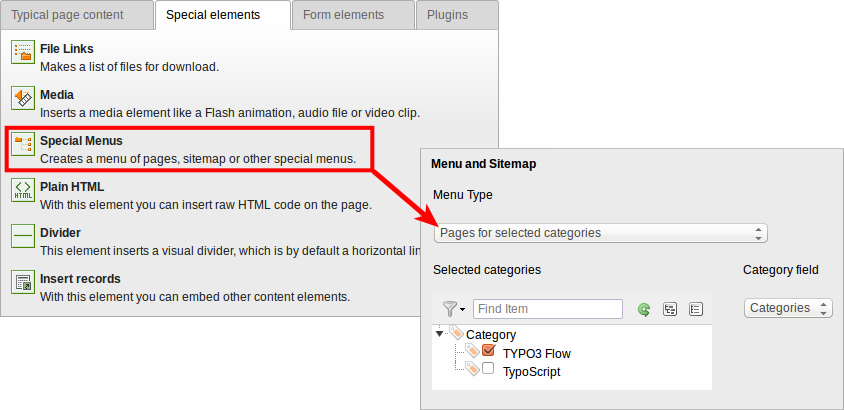
\includegraphics[width=0.8\linewidth]{Images/BackendChanges/CategoryBasedMenus.png}
	\end{figure}

\end{frame}

% ------------------------------------------------------------------------------
% Menu/Sitemap: Category-based Menus
% (slide added in March 2014)
% ------------------------------------------------------------------------------

\begin{frame}[fragile]
	\frametitle{Cambiamenti nel backend}
	\framesubtitle{Menù basato sulle categorie (2)}

	\begin{itemize}
		\item Un'altro nuovo tipo di menù: "\underline{Elementi di contenuto} delle categorie selezionate"
	\end{itemize}

	\begin{figure}
		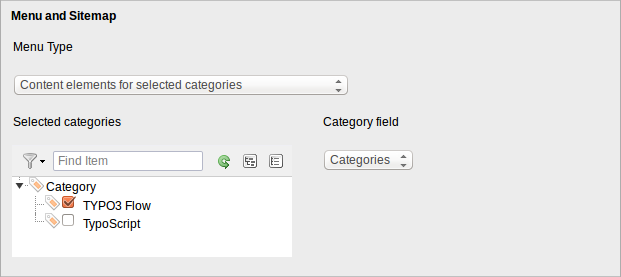
\includegraphics[width=0.6\linewidth]{Images/BackendChanges/ContentElementsForSelectedCategories.png}
	\end{figure}

\end{frame}

% ------------------------------------------------------------------------------
% Sorting Categories
% ------------------------------------------------------------------------------
% http://forge.typo3.org/issues/51590

\begin{frame}[fragile]
	\frametitle{Cambiamenti nel backend}
	\framesubtitle{Ordinamento categorie}

 	\begin{itemize}
		\item Ora le categorie possono essere ordinate\newline
                        \small(in TYPO3 < 6.2, le categorie erano sempre in ordine alfabetico)\normalsize
	\end{itemize}

	\begin{figure}
		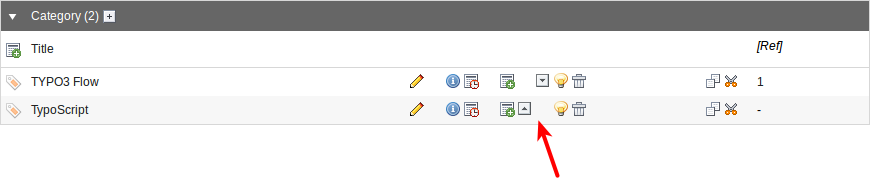
\includegraphics[width=0.95\linewidth]{Images/BackendChanges/CategorySorting.png}
	\end{figure}

\end{frame}

% ------------------------------------------------------------------------------
% Category Visibility
% ------------------------------------------------------------------------------
% http://forge.typo3.org/issues/52718

\begin{frame}[fragile]
	\frametitle{Cambiamenti nel backend}
	\framesubtitle{Visibilità categoria}

 	\begin{itemize}
		\item La visibilità di una categoria può essere limitata ad utenti e gruppi di BE
	\end{itemize}

	\begin{figure}
		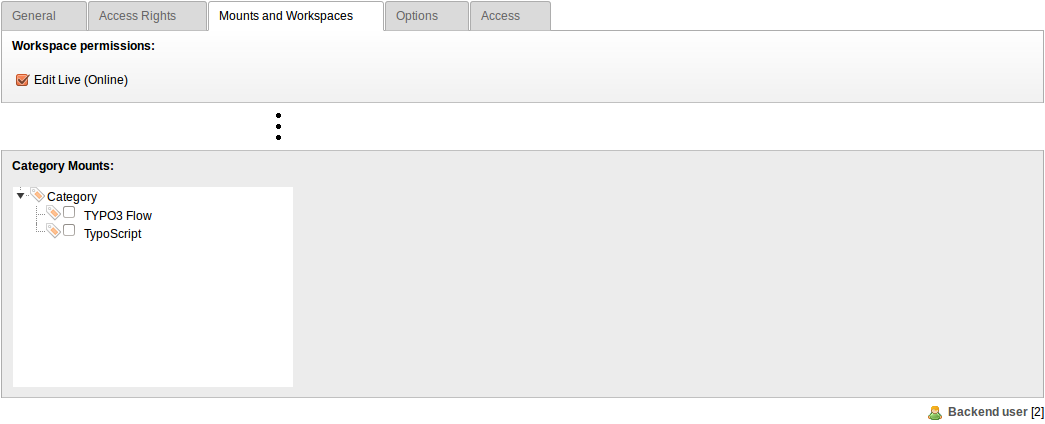
\includegraphics[width=0.95\linewidth]{Images/BackendChanges/CategoryVisibility.png}
	\end{figure}

\end{frame}

% ------------------------------------------------------------------------------
% "New Content" icon always visible
% ------------------------------------------------------------------------------
% http://forge.typo3.org/issues/48938
% http://forge.typo3.org/issues/51480

\begin{frame}[fragile]
	\frametitle{Cambiamenti nel backend}
	\framesubtitle{Usabilità}

 	\begin{itemize}
		\item L'icona "nuovo contenuto" è sempre visibile se la colonna è vuota\newline
			\small(questo aiuta gli editori a capire cosa possono fare)\normalsize
	\end{itemize}

	\begin{figure}
		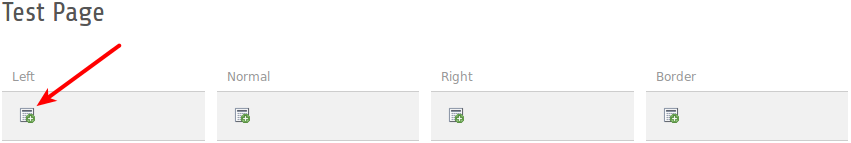
\includegraphics[width=0.95\linewidth]{Images/BackendChanges/NewContentIconAlwaysVisible.png}
	\end{figure}

\end{frame}

% ------------------------------------------------------------------------------
% Module "Functions": Hide In Menus
% ------------------------------------------------------------------------------
% http://forge.typo3.org/issues/51017

\begin{frame}[fragile]
	\frametitle{Cambiamenti nel backend}
	\framesubtitle{Funzioni}

 	\begin{itemize}
		\item Quando si creano pagine multiple nel modulo "funzioni", un nuovo checkbox permette di nascondere queste pagine nel menù\newline
			\small(molto utile, quando si creano varie pagine contemporaneamente)\normalsize
	\end{itemize}

	\begin{figure}
		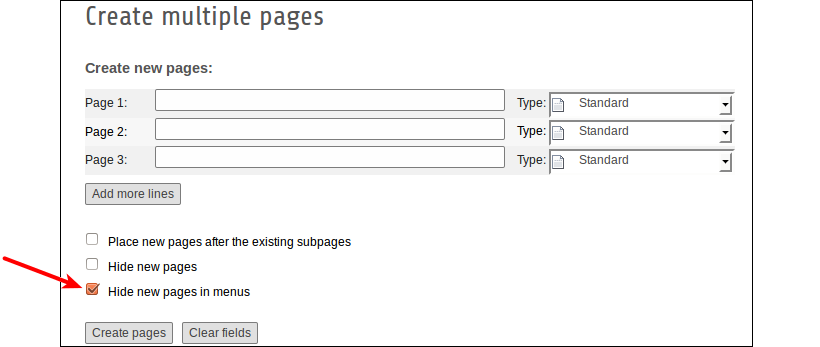
\includegraphics[width=0.85\linewidth]{Images/BackendChanges/CreateMultiplePagesHideInMenu.png}
	\end{figure}

\end{frame}

% ------------------------------------------------------------------------------
% Extension Manager: Upload Extensions
% ------------------------------------------------------------------------------
% http://forge.typo3.org/issues/51776
% http://forge.typo3.org/issues/51437

\begin{frame}[fragile]
	\frametitle{Cambiamenti nel backend}
	\framesubtitle{Extension Manager}

 	\begin{itemize}
		\item Caricamento di un estensione nella funzionalità "Scarica estensioni"
	\end{itemize}

	\begin{figure}
		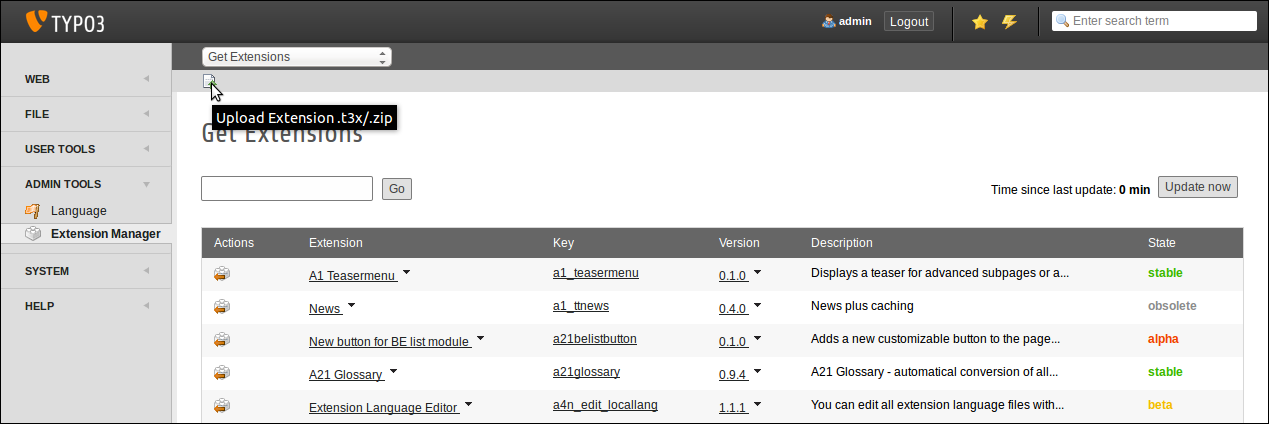
\includegraphics[width=0.95\linewidth]{Images/BackendChanges/UploadExtension.png}
	\end{figure}

\end{frame}

% ------------------------------------------------------------------------------
% Recycler
% ------------------------------------------------------------------------------
% http://forge.typo3.org/issues/52324

\begin{frame}[fragile]
	\frametitle{Cambiamenti nel backend}
	\framesubtitle{Recycler}

 	\begin{itemize}
		\item I record cancellati possono essere ordinati per timestamp\newline
			\small(questo aiuta gli utenti a decidere se recuperare uno specifico record o meno)\normalsize
	\end{itemize}

	\begin{figure}
		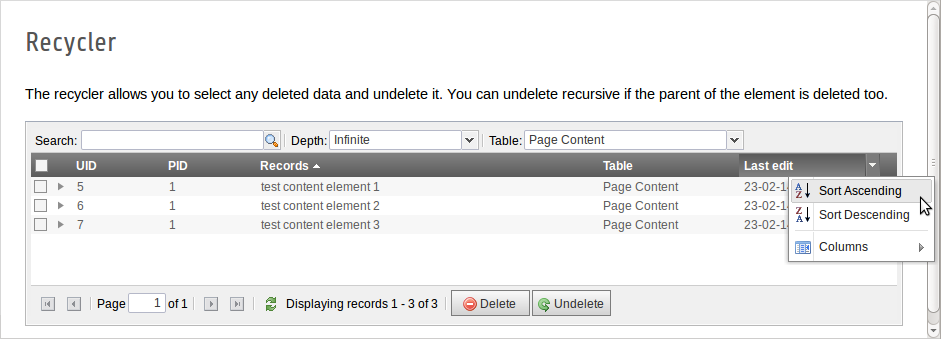
\includegraphics[width=0.95\linewidth]{Images/BackendChanges/RecyclerSortRecord.png}
	\end{figure}

\end{frame}

% ------------------------------------------------------------------------------
% File/Directory Permissions
% ------------------------------------------------------------------------------

\begin{frame}[fragile]
	\frametitle{Cambiamenti nel backend}
	\framesubtitle{Permessi di File/Directory}

 	\begin{itemize}
		\item Molto più granulari i permessi di file/directory per gli utenti/gruppi di backend
			\begingroup\color{typo3red}\textbf{(1)}\endgroup
		\item Questo era possibile da TYPO3 6.0, ma solo tramite UserTSconfig
			\begingroup\color{typo3red}\textbf{(2)}\endgroup
	\end{itemize}

	\begin{figure}
		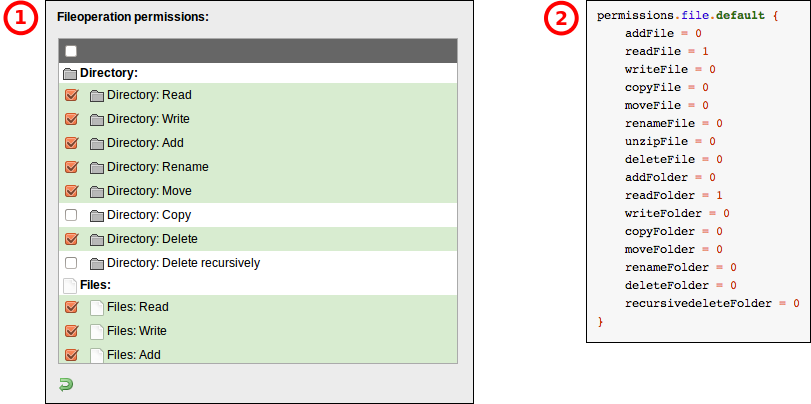
\includegraphics[width=0.75\linewidth]{Images/BackendChanges/FileAndDirectoryPermissions.png}
	\end{figure}

\end{frame}

% ------------------------------------------------------------------------------
% OpenID
% ------------------------------------------------------------------------------

\begin{frame}[fragile]
	\frametitle{Cambiamenti nel backend}
	\framesubtitle{OpenID (1)}

 	\begin{itemize}
		\item L'autenticazione con OpenID per gli utenti di BE può essere configurata usando uno wizard
		\item EXT:openid (estensione di sistema) è necessaria per questa funzionalità
	\end{itemize}

	\begin{figure}
		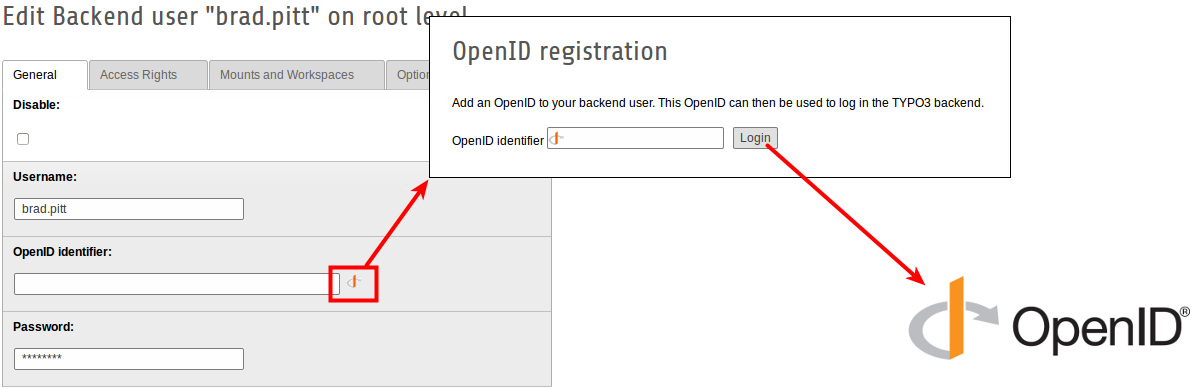
\includegraphics[width=0.95\linewidth]{Images/BackendChanges/OpenIdWizard.png}
	\end{figure}

\end{frame}

% ------------------------------------------------------------------------------
% OpenID
% ------------------------------------------------------------------------------

\begin{frame}[fragile]
	\frametitle{Cambiamenti nel backend}
	\framesubtitle{OpenID (2)}

 	\begin{itemize}
		\item L'autenticazione con OpenID per gli utenti di BE può essere configurata usando uno wizard
		\item EXT:openid (estensione di sistema) è necessaria per questa funzionalità
	\end{itemize}

	\begin{figure}
		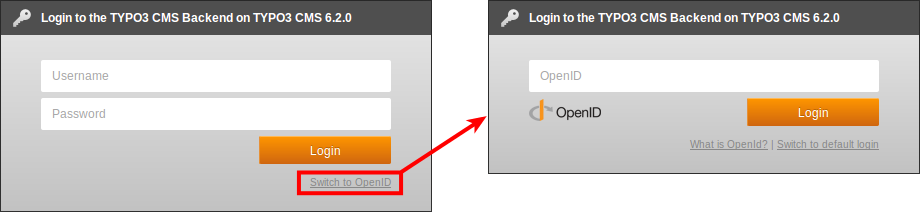
\includegraphics[width=0.8\linewidth]{Images/BackendChanges/OpenIdLogin.png}
	\end{figure}

 	\begin{itemize}
		\item Maggiori dettagli al riguardo di OpenID:\newline
			\small\url{http://openid.net}\normalsize
	\end{itemize}

\end{frame}

% ------------------------------------------------------------------------------
% Workspaces
% ------------------------------------------------------------------------------
% http://forge.typo3.org/issues/50223
% http://forge.typo3.org/issues/50224

\begin{frame}[fragile]
	\frametitle{Cambiamenti nel backend}
	\framesubtitle{Workspaces}

 	\begin{itemize}
		\item Gli editori/utenti possono definire chi avvisare, senza limitazione sul livello di sistema
		\item Il tab "All" è ora visibile a \underline{tutti} gli utenti
	\end{itemize}

	\begin{figure}
		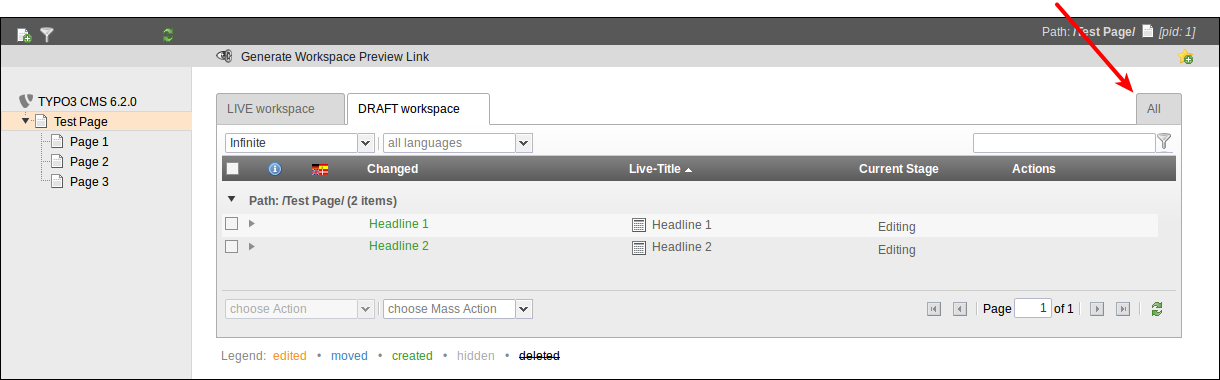
\includegraphics[width=0.95\linewidth]{Images/BackendChanges/WorkspacesTabAll.png}
	\end{figure}

\end{frame}

% ------------------------------------------------------------------------------

